\documentclass{ieeeaccess}
\usepackage{cite}
\usepackage{amsmath,amssymb,amsfonts}
\usepackage{algorithmic}
\usepackage{graphicx}
\usepackage{textcomp}
\usepackage{hyperref}
\hypersetup{
    colorlinks=true,
    linkcolor=blue,
    filecolor=magenta,      
    urlcolor=cyan,
}
\usepackage[ruled,vlined,linesnumbered]{algorithm2e}
\def\BibTeX{{\rm B\kern-.05em{\sc i\kern-.025em b}\kern-.08em
    T\kern-.1667em\lower.7ex\hbox{E}\kern-.125emX}}
\begin{document}
\history{Date of publication March 26, 2021, date of current version March 31, 2021.}
\doi{10.1109/ACCESS.2021.3069114}

\title{Evaluation of Algorithms for Randomizing Key Item Locations in Game Worlds}
\author{\uppercase{Caleb H. Johnson}, 
\uppercase{Jerry L. Trahan, Tao Lu, and Lu Peng}
\IEEEmembership{Senior Member, IEEE}}
\address{Division of Electrical and Computer Engineering, 
Louisiana State University, Baton Rouge, LA 70803, USA}

\markboth
{C. H. Johnson \headeretal: Evaluation of Algorithms for Randomizing Key Item Locations in Game Worlds}
{C. H. Johnson \headeretal: Evaluation of Algorithms for Randomizing Key Item Locations in Game Worlds}

\corresp{Corresponding author: Lu Peng (e-mail: lpeng@lsu.edu).}

\begin{abstract}
In the past few years, game randomizers have become increasingly popular. In general, a game
randomizer takes some aspect of a game that is usually static and shuffles it somehow. In
particular, in this paper we will discuss the type of randomizer that shuffles the locations of
items in a game where certain key items are needed to traverse the game world and access some of
these locations. Examples of these types of games include series such as \textit{The
Legend of Zelda} and \textit{Metroid}. In order to accomplish this shuffling in such a way that
the player is able to reach the end of the game, some novel algorithms in graph theory must be
utilized, where the game world and its item locations are represented as a graph and each edge
on the graph has some rule for which items are required to traverse it. In this paper, we define
these algorithms formally and evaluate them with different metrics that can guide a developer’s
decision about which algorithm works best for their game.
\end{abstract}

\begin{keywords}
Game analysis, game randomization, graph theory.
\end{keywords}

\titlepgskip=-15pt

\maketitle

\section{Introduction}
\label{sec:introduction}
\PARstart{A}{}game randomizer is, in general, a modification of a game that randomizes some
aspect of the game that is usually static. Many kinds of randomizers exist, such as randomizing
enemy encounters, level up rewards, cosmetics, and item locations. In some types of games,
usually belonging to the \textit{Adventure} or \textit{Metroidvania} genres, the player is
required to find some items, abilities, or keys that allow them to move through the game world
and access more locations where items can be found. Therefore, when randomizing the locations of
items in a game like this, there must be some consideration for reachability.

The end goal of randomizing item locations in a game such as this is to ensure that the end of
the game is reachable so that the player is able to complete it. For example, let’s say there is
a hammer item that is able to smash rocks that block the player’s path, and the final area of
the game is guarded by a rock the player must smash to proceed. If the hammer item is placed
hidden underneath a rock, then the player will not be able to access the hammer and thus be
unable to complete the game. Furthermore, let’s say a different item is hidden under that rock,
and that item is required to access the hammer. The result is the same: the game will be
uncompletable.

To accomplish our task of creating a completable placement of items within the game world, the
world will be abstracted to a graph representation. Each node on the graph represents a location
at which an item may be found, and each edge between a pair of nodes defines some rule that is
required to traverse that edge. Utilizing this graph representation and the list of items
currently in the player’s inventory, a reachability graph can be calculated.

\Figure[t!](topskip=0pt, botskip=0pt, midskip=0pt)[scale=0.30]{Figures/johns1.png}
{Detailed view of region and location graph nodes (left), compressed view showing locations as
within regions (right).\label{fig1}}

For the implementation, it will be useful to consider two kinds of nodes on the graph for
organizational purposes: {\it regions} and {\it locations}. A region represents some space
within the game world, such as the interior of a building. A location represents a single point
within a region at which an item can be acquired. In the graph, regions connect to locations
contained within them and to other regions that are directly accessible. Fig.~\ref{fig1} shows
this distinction, with regions and locations as separate nodes on the left and the compressed
view on the right, where a circular node denotes a location and a square node denotes a region.
An important note is that edges between region nodes are not necessarily bi-directional. An edge
could be one way, and oppositely directed edges can have different rules.

We describe three algorithms that utilize this reachability graph to fill empty item locations
in such a way that will produce a completable result: Random Fill, Forward Fill, and Assumed
Fill. Each algorithm has advantages and disadvantages, which will be evaluated in this paper.

Fig.~\ref{fig2} shows an example of a small game world graph that we designed to be similar to a
real game world. Item placements shown here are the "original" placements, designed to be placed
how items would be in a real game world, with key items highlighted in different colors. Refer to
Fig.~\ref{fig1} to understand the meaning of elements of the graph. For example, to travel from 
Forest to Waterfall requires the sword item, and location Chest in Waterfall requires the sling. 
The player would start in Forest, in the top right, and eventually make their way to Arena 
(second to the left from the bottom right) where the goal item is located. One can hand-trace 
a path through this world to eventually complete the game, travelling from region to region and
collecting available item locations. Fig.~\ref{fig3} shows this same world but with the item 
locations randomized by Assumed Fill. One can still trace a path through this graph from the 
starting region to eventually be able to reach the goal and complete the game.

\Figure[t!](topskip=0pt, botskip=0pt, midskip=0pt)[scale=0.41]{Figures/johns2.png}
{An example world graph with original item placements.\label{fig2}}

\Figure[t!](topskip=0pt, botskip=0pt, midskip=0pt)[scale=0.41]{Figures/johns3.png}
{The same example world graph as Fig. 2 with item placements randomized by Assumed
Fill.\label{fig3}}

While we will use the term “item” for anything in the game that can be relocated and “key item”
for an item that can be used to access new locations, within the game itself the item could be
any number of things: a key, an ability, an upgrade, a tool, etc.

Currently, most game randomizers exist as unofficial ROMHacks (modifications made to a 
compiled game executable which is distributed on Read Only Memory) of existing games. 
A recent game, \textit{Bloodstained: Ritual of the Night}, includes a built-in randomizer.
An older game, \textit{Axiom Verge}, recently added a randomizer mode that started 
as a fan-made modification.
As their popularity grows, more games that explore a world unlocking paths by collecting items
could begin to incorporate randomizers as optional modes or even the main mode.

Game players can enjoy randomizers for several reasons. They are somewhat of a mid-point between
adventure games, which typically have low randomization, and games where the entire world is
randomized each playthrough. It ensures that every playthrough is unique, while at the same time
allowing the player to have prior knowledge of the world's layout and rules and where to look to
make progress. They are popular both among casual players who simply want to replay a familiar
game with a new experience, and racers or speedrunners who want to play the game repeatedly to
beat it as fast as possible and desire a new experience each time. When one plays a randomizer
for the first time, there is usually something of a shock factor that brings joy, such as
finding an endgame item very early or a legendary item in an unassuming location.

Our motivation for this work, besides defining the algorithms used for key item placement
randomization so that one can implement them, is to assess these algorithms with different
metrics in order to show some properties of their behavior and provide some guidelines on which
algorithm works best for the game the randomizer is designed for. However, our work could
potentially have application outside of computer games in other areas which utilize randomized
or changing graphs such as networking, machine learning, or blockchain.

The layout of the rest of this work is as follows. Section II reviews some related work. Section
III describes the three fill/item placement algorithms and several search algorithms in depth
and formally defines them using pseudocode. Section IV describes our method to measure the
complexity of a world and our method for generating world graphs. Section V defines the metrics
that will be used to evaluate the algorithms, including the interestingness measure and its
components. Section VI analyzes the results of these metrics based on the algorithm and world
complexity used. Section VII discusses our work critically and mentions some possible future
work. Finally, section VIII provides some concluding remarks.


\section{Related Work}
Ours is the first work researching algorithms for use in generating randomized item placement in
game worlds, but we do have some related work to review.

Dormans and Bakkes \cite{b1} propose a somewhat similar work which represents a playable game
area as a flowchart rather than a graph. A pair of actions such as finding a key and then using
that key to open a door are represented as finding the key being a step in the flowchart before
the step of opening a door. In that sense this work also considers key items which must be
acquired before accessing certain locations. However this paper is more focused on sequences of
actions and generating such sequences to dynamically create enjoyable mission experiences in
games and does not have consideration for changing the order of actions in a world which has
already been created. Their mention of placing items where they will be needed soon also
inspired the idea of the satisfyingness metric, one of the components of interestingness.

Cook and Raad \cite{b2} abstract actions that must be performed within a game to complete a
level into a graph. However there are no edge rules in this graph which lock certain edges, and
no consideration for reachability. The authors of this work find it useful to group some nodes
together into hypernodes, similar to our method of grouping item location nodes into region
nodes which are connected to each other.

Karavolos {\it et al.} \cite{b3} also abstract a game world as a graph, where nodes represent
rooms, edges represent doorways between rooms, and a the value on a node represents what type of
room it is in order to model dungeons in games. However, this work's focus is on generating
graphs to make interesting dungeons to explore without consideration for locked edges and
reachability. This paper instead had a much bigger influence on our work by their method of
measure interestingness in a generated graph. While our methods of measuring interestingness are
very different form theirs, their overall methodology of scoring different aspects and
aggregating these scores for a final output greatly influenced our interestingness metric.

Liapis {\it et al.} \cite{b4} aim to generate interesting explorable spaces and mentions in
their future work section the possibility of using directed graphs with lock and key mechanisms
traversed with Breadth First Search. Their discussion of explorable spaces where backtracking is
undesirable also influenced the mechanism for which our boredom metric, a component of
interestingness, is measured.

Nugraha {\it et al.} \cite{b5} is a paper which creates a method to automatically place items 
in maps for First Person Shooter games using Convolutional Neural Networks. However, this paper is 
concerned with strategic and interesting placement of items that give the player an advantage for 
action-oriented purposes rather than logical placement for world traversal.

Several other papers inspired the creation of our interestingness metric and its individual
components. Pederson {\it et al.} \cite{b6} gave the basic idea for our fun, challenge, and
boredom metrics, especially their definition of fun where constant progress is being made by the
player. Lehman and Stanley \cite{b7}, mentioning novelty as a metric of evaluating
interestingness of a game, gave the idea to incorporate bias into interestingness as more biased
results for randomized worlds are more predictable. Roberts and Lucas \cite{b8} mention of
desiring a challenge which is not too hard or too easy to measure interestingness influenced our
own challenge measurement where we desire a rate of finding key items which is not too often or
too rarely.

While the fill and search algorithms (besides Playthrough Search) existed before the writing of
this paper, they have not been formally defined anywhere, being discussed mainly in the comments
of open source code files and online chat services used by randomizer developers \cite{b9}
\cite{b10}. Perhaps the best source at the time of writing is a panel by randomizer developers
where they discuss, among other topics related to randomizer development, the placement
algorithms \cite{b11}. 


\section{Algorithm Descriptions}
Here we will formally define the algorithms used in generating and evaluating randomized world
graphs. Subsection II.A describes algorithms used to fill the world graph with item placements
while subsection II.B describes algorithms used to search a graph during and after it has been
filled. 

\subsection{Fill Algorithms}

Also called item placement algorithms, these are the algorithms that are used to fill a given
world graph using a given item set in order to create a completable result. These algorithms
utilize the search algorithms given in the next subsection. Each of these algorithms is given an
input graph G, which includes every location in the world at which an item can be found. A node
in G initially has a null value, indicating that it is empty. When an item is placed in that
node, that item is written to the node's value. Edges in G may require certain key items to
traverse. Some other common variables used in these algorithms include:

\begin{itemize}
    \item R: Graph of reachable locations, a subset of G.
    \item I: Set of key items currently owned, determines R.
    \item I' Set of key items not owned, the complement of I, also called the
    item pool.
    \item Start: The starting node of G, search begins from this point.
    \item Goal: The "end" node of G, reaching this node signifies completing the game. If Goal
    is within R, then the game is completable.
\end{itemize}

There are different kinds of items within a game. Our implementation considers the following
types, in order of decreasing importance:

\begin{itemize}
    \item Goal item: This is the item contained at the goal node that signifies completion of
    the game when collected.
    \item Key (or major) item: This is an item that can allow the player to traverse an edge and
    is thus the main consideration for the fill algorithms.
    \item Helpful item: This is an item that is helpful to the player but does not help them
    toward the goal of completing a game as far as graph traversal is concerned. This can
    include items such as more powerful weapons or HP (Hit Point) improvements which allow 
    the player to take more damage before losing.
    \item Junk item: This is an item that is either not helpful or only temporarily helpful.
    This can include items such as currency or ammo refills. Although our implementation
    differentiates between helpful item and junk items, the algorithms do not utilize this
    distinction. Sometimes, helpful items and junk items are collectively referred to as minor
    items.
\end{itemize}

\subsubsection{Random Fill}
Here is the first and most basic fill algorithm. It works simply by placing each item in a
random location in the world until all items have been placed. After distributing the items, a
check is done to see if the game is completable. If not, the algorithm is repeated until a
completable placement has been generated. It can be surmised that in a complex world it could
take multiple thousands of attempts to complete. Algorithm~\ref{Alg1} describes Random Fill. 
Lines 1 and 3-6 are just for initialization before the loop and on repeat attempts. 
The second while loop beginning on line 7 is where the item placement occurs. 
After that, R is computed to check if it contains the goal. If not the world graph and item 
pool are reset and the placement is attempted again.

Usually when Forward Fill or Assumed Fill are utilized they are used on only the key items and
then Random Fill is used to place helpful and junk items that do not affect completability.

We will now discuss the time complexity. For the fill algorithms, n equals the number of key
items to distribute. Sphere Search is an algorithm that will be discussed more in-depth 
in subsection III.B.3, but for now know that it is an algorithm to check completability of 
an item distribution.

A single iteration of Random Fill takes O(n(|V| + |E|)) time for Sphere Search and O(n) time 
for the remainder, since it must loop once for each item to place in the world.
The best case is only one iteration to compute a correct result.
We must consider the expected performance, however. If the world graph contains |V| 
vertices, then the number of possible orders for filling those locations is |V|!.
The number of completable placements depends on the exact world graph. 
A more complex world will generally have fewer completable placements, 
which is verified in Section VI.
If the number of completable placements is constant,
then the expected time for Random Fill to compute a completable
result is O(|V|!(n(|V| + |E|))).

\begin{algorithm}
\label{Alg1}
\SetAlgoLined
\SetKwInOut{Input}{Input}
\SetKwInOut{Output}{Output}
\Input{~Empty world graph G, item pool I', Goal}
\Output{~Completable world graph G}
 I = Empty\;
 \While{R does not contain Goal}{
    G.Reset()\; 
    I'.Add(I)\;
    I'.Shuffle()\;
    I = Empty\;
    \While{(G has nodes with null value) and (I' is not empty)}{
        g = Random null node in G\;
        i = I'.Pop()\;
        g.Value = i\;
        I.Add(i)\;
    }
    R = SphereSearch(G, Start)\;
  }
  return G\;
 \caption{Random Fill}
\end{algorithm}

\subsubsection{Forward Fill}
Next we consider Forward Fill. This is the first of two algorithms that fill the world
intelligently by considering the rule on each edge, however, it is still fairly simple to
understand and implement. It initializes R to be the set of reachable locations from the
beginning of the game. It then chooses a random item from the item pool I' (line 5)
and places it in a random location within R (line 6), also adding that item to I (line 7). 
This location is then removed from consideration and all locations that become reachable 
are added to R through the generalized search algorithm. This process is repeated until 
all items have been placed. Algorithm~\ref{Alg2} describes Forward Fill.

Like in Random Fill, the while loop iterates for each item given, and for our time complexity
consideration n equals the number of key items to distribute. However each iteration must also
perform the search algorithm, which itself has a complexity of O(|V|+|E|) as it is a
modification of Breadth First Search (see Section III.B). 
Therefore the time complexity of Forward Fill is
O(n(|V|+|E|)).

\begin{algorithm}
\label{Alg2}
\SetAlgoLined
\SetKwInOut{Input}{Input}
\SetKwInOut{Output}{Output}
\Input{~Empty world graph G, item pool I', Goal}
\Output{~Completable world graph R}
    I = Empty\;
    I'.Shuffle()\;
    \While{(R has nodes with null value) and (I' is not empty)}{
        r = Random null node in R\;
        i = I'.Pop()\;
        r.Value = i\;
        I.Add(i)\;
        R = Search(G, I, Start)\;
    }
    Return R\;
 \caption{Forward Fill}
\end{algorithm}

\subsubsection{Assumed Fill}
Finally we will consider Assumed Fill. This is the most complex algorithm to understand and
implement, as well as having the highest time complexity for a single iteration. Assumed Fill
begins by assuming the player initially has access to all items, meaning reachable locations R
is equal to the entire world graph G (line 4). In the inverse of the other two algorithms, I is thus
initialized to the set of all items and I' is set to be empty (lines 1-3). A random item
is removed from I in line 6, meaning that R will shrink (rather than expand as it does in Forward Fill).
A random empty location that is still reachable is then selected and the item is placed there 
(lines 8 and 9). The way this algorithm begins by assuming the player has all items and removes 
them can be thought of as the opposite of Forward Fill. Algorithm~\ref{Alg3} describes Assumed Fill.

Assumed Fill does come with a special consideration for its search function, as to work fully it
must account for the case where an item is removed from I but is still within R. This will be
looked at more closely in the following subsection where we define the search algorithms.

Like Forward Fill, the while loop iterates once per each key item and each iteration must
perform the search function. However, Assumed Fill's modified search executes multiple search
iterations (see Section III.B), up to the same number of key items given, 
adding another degree onto Assumed Fill's
time complexity, which is thus O(n\textsuperscript{2}(|V|+|E|)).

\begin{algorithm}
\label{Alg3}
\SetAlgoLined
\SetKwInOut{Input}{Input}
\SetKwInOut{Output}{Output}
\Input{~Empty world graph G, item pool I', Goal}
\Output{~Completable world graph R}
    I = I'\;
    I.Shuffle()\;
    I' = empty\;
    R = G\;
    \While{(R has nodes with null value) and (I is not empty)}{
        i = I.Pop()\;
        R = AssumedSearch(G, I, Start)\;
        r = Random null node in R\;
        r.Value = i\;
        I'.Add(i)\;
    }
    Return R\;
 \caption{Assumed Fill}
\end{algorithm}

\subsection{Search Algorithms}

Now we will consider the search algorithms that the fill algorithms use and that we use to
analyze the resulting filled game worlds. 
The first three are utilized when generating a filled world graph and checking the result and
function as an algorithmic search is expected to work. The last is meant to be an approximation
of a player moving through the game world in order to calculate some information about how a
generated world would feel to play.

\subsubsection{Generalized Reachability Search}

First we consider our generalized search algorithm which computes a reachability graph given an
input world graph, set of items currently owned, and the starting node. This algorithm is
basically a modification of Breadth First Search that checks if an edge is traversable before
adding to the queue the node to which that edge leads on line 10. Edges that are traversable and nodes
which are reachable are added to an initially empty graph in order to construct a full
reachability graph, which is then returned. Algorithm~\ref{Alg4} shows this reachability search.

As this algorithm is a modification of Breadth First Search, it has the same time complexity of
O(|V|+|E|), assuming the lookup time of visited nodes is equal to O(1). 
This could be accomplished with an array of Booleans indicating whether each node has been visited.

\begin{algorithm}
\label{Alg4}
\SetAlgoLined
\SetKwInOut{Input}{Input}
\SetKwInOut{Output}{Output}
\Input{~World graph G, owned items I, Start}
\Output{~Reachability graph R}
    R = Empty\;
    Queue = Empty\;
    Queue.Enqueue(Start)\;
    Visited = empty\;
    Visited.Add(Start)\;
    \While{Queue is not empty}{
       r = Queue.Dequeue()\;
       \For{edge in r}{
            target = node edge leads to\;
            \uIf{RequirementsMet(edge, I) and (Visited does not contain target)}{
                Queue.Enqueue(target)\;
                Visited.Add(target)\;
            }
            \ElseIf{not RequirementsMet(edge, I)}{
                r.Remove(edge)\;
            }
       }
       R.Add(r)
    }
    Return R\;
 \caption{Search}
\end{algorithm}

\subsubsection{Assumed Search}

Assumed Fill utilizes a slight modification of the generalized search algorithm as it must
consider the case when an item has been removed from I but is still within R. Therefore it
utilizes the generalized search algorithm to find a reachability graph, takes any items found
within, then runs the search again (loop starting line 1). Further iterations of finding items 
within R may expand R more, meaning Assumed Search could potentially run as many times as there 
are key items placed within it, so the complexity of this algorithm is the number of items n 
multiplied by the complexity of the general search algorithm, O(n(|V|+|E|). 
Algorithm~\ref{Alg5} shows Assumed Search.

\begin{algorithm}
\label{Alg5}
\SetAlgoLined
\SetKwInOut{Input}{Input}
\SetKwInOut{Output}{Output}
\Input{~World graph G, owned items I, Start}
\Output{~Reachability graph R}
    \While{NewItems is not empty}{
       R = Search(G, I, Start)\;
       NewItems = R.GetItems() - I\;
       I.Add(NewItems)\;
    }
    Return R\;
 \caption{Assumed Search}
\end{algorithm}

\subsubsection{Sphere Search}
Now we will discuss sphere search. This algorithm is given a world that has already been filled
and an initially empty item set I. The goal of this algorithm is to produce a list of
reachability graphs, called spheres, which iteratively discover reachable locations. 
So sphere 0 will contain all locations reachable from the beginning of the game,
sphere 1 will contain all locations reachable with items obtained in sphere 0, etc.
This list is called S. This task is accomplished, somewhat similar to Assumed Fill, 
by performing the generalized search, adding all new items from that search, and repeating this
process until an iteration is performed in which no new locations are discovered. This 
indicates the search has either reached a dead end or all locations have become reachable
(including the goal node). Algorithm~\ref{Alg6} shows Sphere Search.

There are two main purposes for this algorithm. The first is simply to check whether a world
placement is completable by checking if the goal node is contained within the last sphere in
the list. While the goal node could be discovered before the last sphere, each sphere is a
subset of the following sphere, so if it's discovered at all it will be in the final sphere.
The second is to produce a list of progress locations that the player can access in the same
order to complete the game, something of a guide for how they can complete the game if they get
stuck, though it will rarely be the most efficient path through the game.

The following text is an example of a sphere search tracing an output to the end of the game
world shown in Fig.~\ref{fig3}. While each sphere contains all location-item pairs from the
previous spheres, sphere lists are usually printed such that only location-item pairs that are
new in each sphere are displayed.

\begin{verbatim}
Sphere 0:
Field_Hidden A: Bow
Valley_Hidden A: Bombs
City_Quest: GrapplingHook

Sphere 1:
Field_Hidden B: Sword
River_Hidden A: Key

Sphere 2:
Waterfall_Quest: Sling

Sphere 3:
Waterfall_Chest: GateKey

Sphere 4:
Dungeon_Chest: Magic

Sphere 5:
Lake_Quest: Key

Sphere 6:
Arena_Boss: Goal
\end{verbatim}

\begin{algorithm}
\label{Alg6}
\SetAlgoLined
\SetKwInOut{Input}{Input}
\SetKwInOut{Output}{Output}
\Input{~World graph G, Start}
\Output{~List of spheres (graphs) S}
    S = Empty\;
    I = Empty\;
    \While{new locations discovered}{
       s = Search(G, I, Start)\;
       NewItems = s.GetItems() - I\;
       I.Add(NewItems)\;
       S.Add(s)\;
    }
    Return S\;
 \caption{Sphere Search}
\end{algorithm}

As sphere search must iterate potentially once for each item and each iteration performs the
general search algorithm, its time complexity equals O(n(|V| + |E|)). This is the same as
assumed search. Assumed search and sphere search have very similar functionality, but produce
different results.

\subsubsection{Playthrough Search}
The final search algorithm we will consider is Playthrough Search. This algorithm is not
utilized within the fill algorithms but is instead used to extract some metrics about how a
playthrough of a certain world graph may look in order to determine how interesting that
placement of items is. Playthrough Search thus attempts to act as a player would when
traversing the game world. 

It was mentioned in the introduction that we consider two types of nodes on the graph, regions
and locations. A region is a space within the game world, such as a room or a town, while a
location is a single point within that space that contains an item. The previous algorithms
were agnostic to this distinction, considering only locations. However, for a playthrough, this
differentiation is useful. The player will exist within a certain region, collect all locations
available to them within that region, and then move to the next region and collect all
locations there. In order to decide which region the player should move to next, a heuristic is
used. We will first consider the algorithm with a generic heuristic. Algorithm~\ref{Alg7} shows
Playthrough Search. Each iteration of the while loop is one traversal. Items are collected
during this traversal and the heuristic is used to determine which region the player
will occupy on the next traversal (lines 5 and 6).

The heuristic is used to determine which region the player would most strongly desire to move
to next. The heuristic function returns a list of scores for each edge leading from the current
region to a different region. The region that has the maximum score is then set as the current
region for the next iteration of the loop.

\begin{algorithm}
\label{Alg7}
\SetAlgoLined
\SetKwInOut{Input}{Input}
\Input{~World graph G, Start}
    Current = Start\;
    I = Empty\;
    \While{world has available locations that have not been checked}{
       I.Add(all available locations within Current)\;
       ScoreList = Heuristic(G, Current.Edges, I)\;
       Current = Region led to by edge with max score\;
    }
 \caption{Playthrough Search}
\end{algorithm}

This algorithm has a couple of uses. Like sphere search, it can be used both to determine if a
given world is completable and to extract a sequence of item collections that will lead to the
completion of the game. It could be argued that this sequence is more useful than that given in
sphere search since it behaves closer to a player. It can also be used to extract metrics from
the playthrough that can be utilized to determine properties of the given placement of items,
mainly how interesting it is. These metrics will be discussed more in depth in Section V.

We will now define the heuristic we used for our implementation of this algorithm. This
heuristic was created with the following assumptions of the player, which are typical of
players of randomizers \cite{b12}.

\begin{enumerate}
    \item The player has complete knowledge of the game world, so they always know where
    available item locations they have not yet searched can be found.
    \item The player will consider both the number of available locations in each direction as
    well as proximity of these locations when deciding to which region to travel next.
    \item The player will attempt to avoid backtracking and instead be more likely to seek out
    new regions or regions that have been visited less recently.
    \item The player is more likely to visit a region if it is a "dead end", meaning it has
    only a single edge that is attached to the current region. In terms of the game, this would
    be like poking into a single-room building quickly to grab something.
\end{enumerate}

Based on these assumptions, our heuristic uses the following rules to score every exit attached
to the current region by considering the world graph as a whole, which locations have already
been searched, and which locations are available with the given item set. Numbers used within
these rules were fine-tuned through experimentation to give traversals that were reasonable to
player behavior and reactive to different item placements.

\begin{itemize}
    \item The heuristic will search each edge using Depth First Search. Each region visited
    will receive an individual score that equals the number of available, non-empty (not yet
    searched) locations in that region divided by the distance from the current region.
    However, this divider maxes out at 8, so that regions far away are not completely
    discounted if they contain a cluster of many available locations. The exit's score is then
    set to the sum of these individual scores. This satisfies assumptions 1 and 2.
    \item A list keeps track of every region visited. The previous 16 visited regions will 
    receive a penalty by their score receiving a divider (minimum 1) equal to 17 - k, when the
    considered region was visited k traversals ago. This means the most recently visited region
    will have its score divided by 16, the 2nd most recently visited region will have its score
    divided by 15, etc. This satisfies assumption 3.
    \item Finally, if the region is a dead end, which is simply found by checking if no other
    edges lead out of the region, it will receive a 2x multiplier so that the player is more
    likely to check it. This satisfies assumption 4.
\end{itemize}

For an example of this heuristic, see Fig. 4. Exit C will be visited first as it has the
highest score, then move back to start. The scores will then be evaluated again but exit C's
score will be 0 as all of its available locations have been searched. Exit A will then win
instead, because although the path through exit A visits the same regions as exit B, exit A has
more locations in closer proximity. After moving through the three regions in the upper right,
the search will finally move toward exit D and fully search all locations within this graph.

\Figure[t!](topskip=0pt, botskip=0pt, midskip=0pt)[scale=0.30]{Figures/johns4.png}
{Example of our heuristic for Playthrough Search. The number in each region shows the number of
available locations in that region.\label{fig4}}

\section{World Complexity and Generation}
For this research, we want to not only study the properties of the output and performance of
the different fill algorithms, but also study the effect the world itself can have on these.
The size and complexity of a game world can vary greatly, from small games that take only a few
hours to complete to games that are expected to take 40+ hours to finish. Therefore we must
have some way to measure the complexity of a given world graph. This section goes over how we
accomplish this, as well as our method of generating randomized worlds to use for testing
purposes.

\subsection{Individual Location Complexity Score}
When normally assessing the complexity of a graph, one may consider the number of nodes and
edges. For our purposes, complexity is less a representation of the size of the graph and more
of how difficult it is to move through the graph. We expect a more complex world to have a
higher chance to fail to generate a completable placement for Random Fill, as the likelihood
of an acceptable placement decreases. Therefore we must create our complexity measure so that
it considers the rules on each edge of the graph.

To accomplish this, we observe each location within the game world and construct what we call a
\textit{total rule}. A total rule includes not only the rule on the edge between a location and
its encompassing region, but also all of the rules that are required to reach that region.
Thus, we set a total rule for each location that incorporates the location's individual rule
AND the rule for each path to that region. The rules along the path from the start region to
the target region are ANDed to create a path rule, and each of these path rules are ORed. 

For a location $L$ contained within an encompassing region,
let $p_i = \langle r_{i,0}, r_{i,1}, \ldots, r_{i,k(i)} \rangle$
denote the $i$th path from the start region to the
encompassing region, where $r_{i,0}$ is the start region and
$r_{i,k(i)}$ is the encompassing region.
Let $q$ denote the number of such paths, and let $RelativeRule$
denote $L$'s rule relative to its encompassing region.
The total rule for a location $L$ can be represented by the following formula:
\begin{equation}
RelativeRule \wedge \bigvee_{i=0}^{q-1}
\bigwedge_{j=1}^{k(i)}rule\;from\;r_{i,j-1}\;to\;r_{i,j}
\label{eq_total_rule}
\end{equation}
An example of this can be seen graphically in Fig. \ref{fig5}.

\Figure[t!](topskip=0pt, botskip=0pt, midskip=0pt)[scale=0.40]{Figures/johns5.png}
{Example of formula for a total rule.\label{fig5}}

These paths are calculated using Depth First Search and once the total rule is found, it is
simplified with Boolean statement simplification methods. Each total rule is then scored using
the following criteria:

\begin{itemize}
    \item Start with each rule having a base complexity of 1
    \item Each key item requirement adds 1 to the complexity
    \item An AND adds .5 complexity since it makes the rule harder to satisfy
    \item An OR subtracts .5 complexity since it makes the rule easier to satisfy
\end{itemize}

By doing this calculation on each location within the world graph, a list of individual
location scores can be obtained. But now the question is how to calculate a final score given
this list of scores. After some thorough evaluation utilizing the world generation, we decided
to take the average of the top 50\% of individual scores to produce the final complexity score.
Using the top 50\% makes it so having many easy to reach locations near the beginning of the
game world does not obscure the true complexity of the harder to reach areas, which is what
really determines how difficult it is to move through the game world. We decided against
summing these scores as having more locations does not necessarily add complexity, but the
score grows very quickly using this method.


\subsection{World Generation}
For our research we desire a method to generate world graphs given a couple of baseline inputs.
These generated worlds were originally used to evaluate different possible metrics for scoring
complexity but their main use is for testing purposes. We will now describe our generation
process.

The world generator is passed two arguments: 
number of regions to generate and number of key items. 
It begins by generating a list of regions (named Region-0, Region-1, Region-2, etc.) and a list
of key items (named simply A, B, C, etc.). 
The first region is designated as the start region, the second region is generated as the hub
region (a very common practice in game design is to have a hub region) and the final region is
designated as the goal region.
Each edge and item will have a rule composed of no, one, or more requirements.

If two regions are directly connected,
then they will have a pair of oppositely directed edges
between them.
For simplicity, these edges' rules will be equal.
For each type of region, we describe below the creation of 
certain outgoing edges and their rules.
For each such edge, Table \ref{table1} gives the probability distribution of 
requirements for the rule for the pair of incoming and outgoing edges.

The start region is generated in the following manner. It is guaranteed to have an outgoing
edge (exit) to the hub region with no requirement, an outgoing edge to a random region with one
item requirement, and a 50\% chance of an outgoing edge to a third region with a 50\% chance
between having no requirement or requiring a single item. It is also generated containing three
item locations with no requirement and a 50\% chance of a fourth location with one requirement.

The hub region also has special rules for generation. It will always generate with six outgoing
edges, three of which have no requirement (one of these leads to the start region) and three
which have a single requirement. It also generates with two item locations with no requirement,
one with one requirement, and one with two requirements.

The final region has no special rules for number of outgoing edges but each incoming edge will
require every key item in the world to traverse. While a game may not necessarily require every
key item to reach the end, typically most if not all are required. The final region will also
contain a single item location, which contains the goal item, the collection of which signifies
completion of the game.

Other regions are generated in the following manner. Each will generate one or two outgoing
edges (50\% chance of each) with a random rule according to Table \ref{table1} and will allow a
maximum of four outgoing edges including edges generated by other regions.
(Note:  When a region generates an outgoing edge to a random destination region, it considers
only regions with fewer than four connections as possible destinations.)
Each region will generate two, three, or four (each equally likely) item locations with a
randomly generated rule.

Rules are randomly generated in the following manner. A one requirement rule will simply choose
a single key item from the item list that will be the requirement. A two requirement rule will
choose two key items (not the same one) and have a 50\% chance each for them to be joined with
AND or OR. A three requirement rule just generates a two requirement rule and a one requirement
rule (making sure the item in the one requirement rule is not redundant with the two
requirement rule) and again randomly joins them with either AND or OR.

There is also a chance to generate a complex requirement. A complex requirement will generate
two or three (50\% chance each) clauses, where a clause has a 20\% chance to be a single
requirement, and a 40\% chance each to require two or three items joined by a random selection
of AND or OR.

The distribution of requirement probabilities for item locations and edges is shown in Table
\ref{table1}. We decided that edges should be more generous since an exit (outgoing edge) is
often simply an open doorway the player can freely walk through.

\begin{table}
\caption{Chance of Generating Each Type of Rule for Item Locations and Edges}
\label{table1}
\setlength{\tabcolsep}{3pt}
\renewcommand{\arraystretch}{1.2}
\begin{tabular}{ |p{100pt}|p{60pt}|p{60pt}|  }
 \hline
 Rule Type & Item Location & Edge \\
 \hline
 No Requirement & 20\% & 60\% \\
 \hline
 One Requirement & 40\% & 20\% \\
 \hline
 Two Requirements & 20\% & 10\% \\
 \hline
 Three Requirements & 10\% & 5\% \\
 \hline
 Complex Requirement & 10\% & 5\% \\
 \hline
\end{tabular}
\end{table}

After all of the previous steps, two finalizing steps are performed. First, we make sure the
graph is connected by checking if all regions have a path to them from the start region. If
not, more edges are added to make the graph connected. Next, a number of junk or helpful items
(50\% chance of each) equal to the number of generated locations minus the number of key items
are generated and added to the item list. This ensures that there is a possible item for every
location in the game world. We believe our method produces worlds which are comparable to 
real game worlds \cite{b1}.

\subsection{Worlds Generated for Algorithm Evaluation}
Using our world generation method, we generated five worlds of increasing complexity to use in
testing. Table \ref{table2} shows some properties of these worlds. Keep in mind that the region
count and item count were input parameters to the generation, while the number of item
locations and the final complexity score were a result of the generation. These input
parameters were chosen to give increasing complexity in a desirable manner.

\begin{table}
\caption{Testing World Properties}
\label{table2}
\setlength{\tabcolsep}{3pt}
\renewcommand{\arraystretch}{1.2}
\begin{tabular}{ |p{35pt}|p{45pt}|p{45pt}|p{40pt}|p{45pt}|  }
 \hline
 Name & Region Count & Item Count & Locations & Complexity\\
 \hline
 World 1 & 10 & 5 & 26 & 4.31 \\
 \hline
 World 2 & 25 & 10 & 74 & 11.11 \\
 \hline
 World 3 & 35 & 15 & 105 & 22.25 \\
 \hline
 World 4 & 45 & 20 & 135 & 32.63 \\
 \hline
 World 5 & 50 & 30 & 143 & 53.23 \\
 \hline
\end{tabular}
\end{table}

To ensure these worlds were not outliers, 100 worlds with the same input parameters were
generated and their average complexity calculated. The worlds used here had complexity within
10\% of these average values.

\section{Description of Algorithm Evaluation Metrics}
In this section we will define the different metrics by which we evaluate the algorithms'
performance and results.

\subsection{Failure Rate}
Defining failure as generating a world that is not completable,
all of our item placement algorithms have a chance of failure.
Random Fill can fail many times before producing a successful result. Forward and Assumed Fill,
on the other hand, should almost never fail, although they can in certain situations. Fig.
\ref{fig6} shows an example of a situation where Forward Fill may be very likely to fail. Since
the start region leads from a single edge locked by Item A and has only three available
locations, if Item A is not one of the first three items selected to be placed, then the
algorithm would fail. In a situation like this, a randomizer developer may choose to hard-code
it such that Item A is placed before any other items to avoid failure. 

\Figure[t!](topskip=0pt, botskip=0pt, midskip=0pt)[scale=0.30]{Figures/johns6.png}
{Example of a graph where Forward Fill is likely to fail.\label{fig6}}

While we expect the failure rate for Forward and Assumed Fill to be very small to the point of
being almost negligible, we expect the failure rate of Random Fill to grow quickly 
as the complexity of the graph increases, which is supported by our results in Section VI.

\subsection{Execution Time}
For each iteration of each algorithm on each test world we will measure the execution time to
complete that iteration. We expect that for a single iteration, the increasing order of
execution time will be Random, Forward, then Assumed Fill. We also expect the execution time to
increase as world complexity increases.

For the fill algorithms, however, we have another consideration for execution time, that is the
failure rate. Especially for Random Fill, the time of a single iteration does not tell the
whole story if the algorithm must potentially be run multiple times to produce a completable
result. Therefore we will also compute an expected execution time that multiplies the execution
time for a single iteration by the reciprocal of the success rate, which is simply 1 minus the
failure rate. This gives the expected time to produce a completable world placement. For
example, if an algorithm has a 50\% failure rate, then it is expected that it will have to be
run twice to generate a successful placement, so we multiply the execution time for a single
iteration by 2. We expect that the adjusted execution time will go in increasing order of
Forward, Assumed, then Random Fill. However, for the less complex worlds there is possibly a
chance that Random Fill could still be faster than the others.

\subsection{Bias}
Bias is the propensity of a fill algorithm to cluster more key items together, in terms of
progress through the game world, typically toward the beginning of the game. Basically, in an
algorithm such as Forward Fill, the first several spheres of a sphere search are likely to
contain a disproportionately high number of key items.

The calculation of bias is fairly simple. After a successful world placement is generated, a
sphere search is performed. (This could be done on an unsuccessful placement as well, but this
would not be a very relevant or helpful metric.) Each sphere subtracts the fraction of new
locations within that sphere (relative to the total number of locations in the game world) from
the fraction of new key items in that sphere (relative to the total number of key items). The
absolute value of this number is added to a sum for each sphere. (If absolute value was not
taken, the sum would always equal 0 by the end.) This sum is then divided by the number of
spheres for normalization. This value then gives a good general idea for how clustered together
the key items are in the overall progression.

We will also measure a bias direction, by keeping separate sums before and after the middle
sphere that do not take the absolute value of each sphere's individual bias. By checking which
sum (the sum before or after the middle) is higher, it can be determined if the bias is more
toward the beginning or more toward the end of the game progression. We expect it to almost
always be toward the beginning, especially for Forward Fill.

Bias is a metric that has been discussed by randomizer developers before the writing of this
paper as a reasoning to use one algorithm over another. It is also a very objective measure
compared to interestingness and its other metrics as it does not utilize the somewhat
subjective PlaythroughSearch to calculate its result. However, ours is the first work to
quantitatively measure bias as a function of the algorithm used and complexity of the world
graph used.

\subsection{Interestingness}
Interestingness is a metric that attempts to capture the overall quality of a placement by a
numeric score from a generated world graph. Interestingness includes five considerations, each
a floating point number in the range [0, 1] and weighted at 20\% to produce a final value:

\begin{itemize}
    \item Bias (Lower is better)
    \item Fun (Higher is better)
    \item Challenge (Higher is better)
    \item Satisfyingness (Higher is better)
    \item Boredom (Lower is better)
\end{itemize}

Therefore the formula for interestingness is equal to
0.2[(1 – bias) + fun + challenge + satisfyingness + (1 – boredom)].

Bias has already been discussed in the previous subsection. The decision to include bias in
interestingness, considering more biased worlds result in more predictability, was influenced
by Lehman and Stanley \cite{b7}. We will now discuss the other four metrics in depth.  Each of
these four measures is based on information extracted from Playthrough Search on the given
world graph. Numbers used for the calculation of these metrics were fine-tuned through
experimentation to give results within a reasonable range and that varied depending on 
the generation.

The overall idea of utilizing different individual interestingness metrics and aggregating them
to create a final score was influenced by Karavolos {\it et al.} \cite{b3}. 

\subsubsection{Fun}
Fun is a metric meant to represent the player consistently making progress by discovering item
locations. Hopefully at least one location is discovered for every traversal to keep up
consistent progress. From Playthrough Search, we extract a list of how many new locations are
searched per traversal. 

Fun is then calculated in the following manner. A loop goes through this list and maintains a
rolling average of the last five traversals. If this average is greater than or equal to 1, a
true value is added to a list of Booleans. If it is less than 1, a false value is added. This
rolling average gives a better representation for how many items the player is currently
finding, even if they go one or two traversals without finding any during a high rate of
searching, or occasionally find one or two during a low rate. The final score for fun then
equals the fraction of true values within this list.

The idea for measuring fun by the player making constant progress was inspired by Pederson {\it
et al.} \cite{b6}.

\subsubsection{Challenge}
Challenge is a metric to represent the rate at which the player obtains key items (thus
unlocking more of the world) being not too often or too rarely. Playthrough Search gives us a
list of how many traversals the search did between finding each key item. 

Challenge is then calculated as follows. We first get an optimal traversal value by dividing
the number of locations in the world by the number of key items so that our range is relative
to the number of locations in the world. The lower threshold is then set to the floor of 50\%
of this number, while the upper threshold is set to the ceiling of 150\% of this number.
Similarly to the fun calculation, we then iterate through the list and find the fraction of
values in the list within this desirable range (inclusive) using a slightly tighter rolling
average of the last three values. The final challenge score is then this fraction.

The idea for challenge being represented by the rate at which key items were found was inspired
by Pederson {\it et al.} \cite{b6} and the idea that a desirable rate should be within a range
that is not too low or high was given by Roberts and Lucas \cite{b8}.

\subsubsection{Satisfyingness}
Now we discuss satisfyingness. This metric is meant to represent, once the player acquires a
new key item, how satisfying is it to find this. We define satisfying as how immediately useful
the item is, as it feels good for the player if they find something that unlocks a large chunk
of the world at the same time. From Playthrough Search we extract a list of how many new item
locations are unlocked every time a key item is found.

Satisfyingness is then calculated in the following manner. Unlike fun and challenge, it does
not use a rolling average. Like fun and challenge, we set a threshold and look for the
fraction of values in the list that are greater than or equal to this threshold. We set the
threshold to the floor of the number of locations in the world (disregarding those that are
immediately available, since these should not factor into how satisfying it is to unlock new
locations) divided by the number of key items.

Satisfyingness being measured as how immediately useful a key item is at the time it is found
was inspired by Dormans and Bakkes \cite{b1}.

\subsubsection{Boredom}
The final metric for interestingness is boredom. Like bias, lower boredom is better. Boredom
measures regions that are visited more often than usual throughout the playthrough. Our
heuristic for Playthrough Search was constructed to try to avoid backtracking, but more
backtracking is inevitable as world complexity increases. From Playthrough Search we have a
list of how many times each region was visited.

Like the other interestingness metrics besides bias, we inspect each value in this list and set
boredom equal to the fraction of these values greater than (rather than greater than or equal
to, to be slightly more generous) a threshold. Here the threshold is set as the ceiling of the
average number of traversals per region.

The idea to incorporate a boredom metric was given by Pederson {\it et al.} \cite{b6} and
measuring it as the amount of backtracking the player must do to complete the game was
influenced by Liapis {\it et al.} \cite{b4}.

\section{Experimental Results}
In this section we will describe the setup and results of our experimentation to evaluate the
performance and output of each algorithm relative to each other and to the complexity of the
input world graph.


\subsection{Experimental Setup}
Our implementation was coded in C\# and run on a Windows machine with an AMD Ryzen 9 3900x
processor and 32GB of DDR4 RAM. Each algorithm was performed on each of the 5 input worlds
100,000 times (for a total of 1.5 million trials). On each trial, the following information was
recorded within a SQLite database:

\begin{itemize}
    \item Which algorithm was used
    \item Which world was used
    \item Execution time (of the fill algorithm only)
    \item Whether the result was completable
    \item Bias score
    \item Bias direction
    \item Interestingness score
    \item Fun score
    \item Challenge score
    \item Satisfyingness score
    \item Boredom score
\end{itemize}

Randomness is provided by C\#’s default random class, which utilizes Donald E. Knuth’s
subtractive random number generator algorithm. The implementation can be viewed on GitHub
\cite{b13}.

\subsection{Results and Evaluation}

Results for the failure rate are shown in Table \ref{table3}. It can be seen that the failure
rate for Random Fill increases as the complexity of the world increases, except for the change
from World 4 to World 5, where the failure rate actually decreases. On the other hand, Forward
Fill and Assumed Fill have a 0\% failure rate up until World 5, where they both have a very
small percentage of failures, with Forward Fill having more than Assumed Fill.

\begin{table}
\caption{Failure Rate per Algorithm per World (\% Failed)}
\label{table3}
\setlength{\tabcolsep}{3pt}
\renewcommand{\arraystretch}{1.2}
\begin{tabular}{ |p{60pt}|p{30pt}|p{30pt}|p{30pt}|p{30pt}|p{30pt}|  }
 \hline
 Algorithm Used & World 1 & World 2 & World 3 & World 4 & World 5\\
 \hline
 Random Fill & 85.943\% & 97.619\% & 99.488\% & 99.945\% & 99.885\% \\
 \hline
 Forward Fill & 0\% & 0\% & 0\% & 0\% & 0.725\% \\
 \hline
 Assumed Fill & 0\% & 0\% & 0\% & 0\% & 0.002\%\\
 \hline
\end{tabular}
\end{table}

Upon inspection of World 5, it was found that the goal region was placed connected to the hub
region. (While this may seem strange, this is actually not uncommon game design.) Perhaps
having that early edge locked with a very difficult lock made it so Forward Fill was more
likely to get stuck early on when generating item placements. Random Fill, on the other hand,
seemingly benefits from having the final region close to the start of the game.

\begin{table}
\caption{Single-Iteration Execution Time per Algorithm per World (ms)}
\label{table4}
\setlength{\tabcolsep}{3pt}
\renewcommand{\arraystretch}{1.2}
\begin{tabular}{ |p{60pt}|p{30pt}|p{30pt}|p{30pt}|p{30pt}|p{30pt}|  }
 \hline
 Algorithm Used & World 1 & World 2 & World 3 & World 4 & World 5\\
 \hline
 Random Fill & 0.037 & 0.231 & 0.438 & 0.746 & 0.801 \\
 \hline
 Forward Fill & 0.266 & 1.113 & 2.776 & 5.224 & 9.645 \\
 \hline
 Assumed Fill & 0.754 & 4.126 & 14.021 & 26.810 & 63.995 \\
 \hline
\end{tabular}
\end{table}

\Figure[t!](topskip=0pt, botskip=0pt, midskip=0pt)[scale=0.40]{Figures/johns7.png}
{Average execution time per algorithm per world (ms). Lower is better.\label{fig7}}

Next is the execution time, shown in Table \ref{table4} and Fig. \ref{fig7}. It can be seen
that while the time in World 1 is fairly similar for all three algorithms, Assumed Fill quickly
grows in execution time faster than Forward Fill which grows faster than Random Fill. This is
due to Assumed Search requiring multiple searching per fill iteration, shown in the Assumed
Search pseudocode.

Now we will consider the expected execution time, shown in Table \ref{table5} and Fig.
\ref{fig8}. When an expected execution time is calculated by considering the failure rate,
Random Fill is still actually the lowest time expectancy for World 1. In Worlds 2 and 3, Random
Fill’s expected time is larger than either of the other two, but still not obscenely so. World
4 is where the failure rate grows so large that it is hardly comparable to the other two,
taking 1356.6ms compared to Assumed Fill’s 26.8ms, an increase of over 50 times. Because of the
lower failure rate for World 5, the expected execution time for Random Fill in World 5 is
actually less than in World 4, but is still over 10 times that of Assumed Fill.

\begin{table}
\caption{Expected Execution Time per Algorithm per World considering Failure Rate (ms)}
\label{table5}
\setlength{\tabcolsep}{3pt}
\renewcommand{\arraystretch}{1.2}
\begin{tabular}{ |p{60pt}|p{30pt}|p{30pt}|p{30pt}|p{30pt}|p{30pt}|  }
 \hline
 Algorithm Used & World 1 & World 2 & World 3 & World 4 & World 5\\
 \hline
 Random Fill & 0.261 & 9.723 & 85.600 & 1356.551 & 696.269 \\
 \hline
 Forward Fill & 0.266 & 1.113 & 2.776 & 5.224 & 9.716 \\
 \hline
 Assumed Fill & 0.754 & 4.126 & 14.021 & 26.810 & 63.996 \\
 \hline
\end{tabular}
\end{table}

\Figure[t!](topskip=0pt, botskip=0pt, midskip=0pt)[scale=0.40]{Figures/johns8.png}
{Expected execution time accounting for failure rate per algorithm per world (ms). Lower is
better.\label{fig8}}

For the following metrics, only successful placements of items within a world are considered.

First we will look at the bias, shown in Fig. \ref{fig9}. Random and Assumed Fill both having
fairly low and close together bias while Forward Fill having consistently higher bias is
expected. What is somewhat unexpected is that in each case, Assumed Fill actually gives
slightly lower bias than Random Fill. This is a bit unintuitive, but an explanation is that
while Assumed Fill is actively more likely to place key items in the later regions of the game 
(due to the entire world being placeable at the beginning and assumed search ensuring the 
reachability graph does not shrink too quickly),
Random Fill has no such propensity, so whenever considering successful results only perhaps
Random Fill is more likely to produce a successful result when it happens that more items are
placed earlier compared to Assumed Fill. (If not considering successful results only, Random
Fill’s bias is almost 0, but this is not a useful statistic.) It is also shown that, as the
world becomes more complex, bias decreases across the board, likely due to having more
opportunities to place items in the later regions of the game. 

\Figure[t!](topskip=0pt, botskip=0pt, midskip=0pt)[scale=0.40]{Figures/johns9.png}
{Average bias per algorithm per world. Lower is better.\label{fig9}}

When calculating a number for bias, whether the bias was toward the beginning or end of the
game is not considered: It simply calculates a number representing the inequality of
distribution. Therefore while calculating this number we can also perform a check to see
whether this inequality is toward the earlier or later regions of the game, with the former
being much more common in all cases. Fig. \ref{fig10} shows the percentage of time bias was toward 
the end rather than toward the beginning (so, for example, if the value is 5\% then bias was toward 
the end 5\% of the time and toward the beginning 95\% of the time). It can be seen that bias being
toward the end was a somewhat common occurrence for all three algorithms in World 1, being
roughly a 5\% chance for Forward Fill up to an almost 16\% chance for Random Fill. This rate
drops hard in the following worlds, going to almost 0\% for Forward Fill and up to around 3\%
at most for Random and Assumed fill. World 4, in particular, has around 0\% for all three
algorithms, and the overall percentage does not seem to follow any particular pattern as
complexity increases. It can then be assumed that whether the bias is more likely to be toward
the end of the game is more a result of the design of the world itself rather than the
complexity measure. However, it is still shown to be a less likely occurrence using Forward
Fill.

\Figure[t!](topskip=0pt, botskip=0pt, midskip=0pt)[scale=0.40]{Figures/johns10.png}
{Percentage of time bias was toward the end of the game rather than toward the beginning per
algorithm per world.\label{fig10}}

Now we will consider interestingness, shown in Fig. \ref{fig11}. Note the measure on the side
of the graph. All three algorithms are fairly close in their final interestingness score, in
general with Forward Fill producing the least interesting result followed by Assumed which is
very closely followed by Random. However, in World 5 Forward Fill suddenly jumps ahead of both
of them. To understand why this happens, we must look more closely at the individual metrics
composing interestingness. In general, Random Fill and Assumed Fill produce similar results for
the individual metrics, while Forward Fill excels in different areas. Overall, interestingness
falls as the worlds become more complex, likely due to more complex worlds meaning on average
more traversals needed and more time required to make progress, even relative to the number of
regions.

\Figure[t!](topskip=0pt, botskip=0pt, midskip=0pt)[scale=0.40]{Figures/johns11.png}
{Average interestingness per algorithm per world. Higher is better.\label{fig11}}

The graph for the fun metric is shown in Fig. \ref{fig12}. As expected, Forward Fill’s result
is higher than the other two, while Random Fill barely edges out Assumed Fill in all cases. Due
to Forward Fill producing world placements where key items are found earlier, it is easier for
the player to make constant progress collecting item locations as they are less likely to be
held back by a low number of currently owned items. Although the fun metric accounts for total
number of locations when computing its threshold, more complex worlds are more likely to
require the player to traverse for longer periods without checking item locations as they move
around regions that have already been looted to get to ones that have not.

\Figure[t!](topskip=0pt, botskip=0pt, midskip=0pt)[scale=0.40]{Figures/johns12.png}
{Average fun per algorithm per world. Higher is better.\label{fig12}}

Next we will observe the challenge metric in Fig. \ref{fig13}. Random and Assumed Fill are
again very close in this metric, with Assumed Fill barely beating out Random Fill in the first
two worlds and vice versa in the next three. However, the final challenge score seems to mostly
plateau for these two algorithms starting at World 2. Forward Fill, on the other hand, is
overall lower and similarly plateaus at World 2, however it has a sudden jump in challenge at
World 5 that puts it almost even with Assumed Fill. This jump is certainly a large factor as to
why Forward Fill’s final interestingness score beat out the other two in World 5. The reason
for this jump in challenge is likely the same reason Forward Fill had a relatively high failure
rate in World 5.

\Figure[t!](topskip=0pt, botskip=0pt, midskip=0pt)[scale=0.40]{Figures/johns13.png}
{Average challenge per algorithm per world. Higher is better.\label{fig13}}

Next is satisfyingness, shown in Fig. \ref{fig14}. All three algorithms produced similar
results for this metric, especially in World 1, but in all cases with Random Fill having the
best score and Forward Fill having the worst score. The score is also mostly similar across
each world, with the difference from the lowest to highest score being only .059, .135, and
.086 for Random, Forward, and Assumed Fill respectively. Assumed Fill is again closer to the
results of Random Fill than Forward Fill.

\Figure[t!](topskip=0pt, botskip=0pt, midskip=0pt)[scale=0.40]{Figures/johns14.png}
{Average satisfyingness per algorithm per world. Higher is better.\label{fig14}}

Finally we observe the results for boredom in Fig. \ref{fig15}. For this metric, Random and
Assumed Fill’s results are so close together they are practically the same, besides a slight
difference in World 4. Forward Fill is less boring on average, since finding key items earlier
leads to overall fewer traversals as the player is less likely to have to revisit regions after
finding more items to clear them out. As complexity increases, boredom increases as well,
likely for the same reason fun decreases: having a larger world will require more traversals as
the player travels through regions that have already been searched to get to regions that have
not yet been searched.

\Figure[t!](topskip=0pt, botskip=0pt, midskip=0pt)[scale=0.40]{Figures/johns15.png}
{Average boredom per algorithm per world. Lower is better.\label{fig15}}

Overall, Forward Fill’s ability to stay ahead of the other two algorithms in the
decreasing/increasing metrics of fun/boredom, while also having a sudden jump in challenge and
somewhat of a sudden decrease in bias for World 5, allowed it to beat the other two in
interestingness for World 5. While this result is worth noting, it does not necessarily mean
that Forward Fill is the preferred algorithm for more complex worlds. Our method of world
generation is not perfectly representative of a real game world and it is possible that a
differently designed world of similar complexity would still have Random and Assumed Fill get a
higher interestingness score than Forward Fill. 

In general, Random and Assumed Fill perform better when considering bias, challenge, and
satisfyingness, while Forward Fill performs better when considering fun and boredom. While we
calculated interestingness using an equal 20\% share for each metric, different weights could
potentially be used. However, for the most part all that changing these weights would do is
shift the graph to more strongly favor one of Random/Assumed Fill or Forward Fill.


\section{Discussion}
Our goal was to provide generic implementations of the algorithms that did not have
game-specific considerations. For example, while this work was inspired by the randomizer for
\textit{The Legend of Zelda: Ocarina of Time}, this game’s randomizer requires special
considerations for the player’s age (child or adult) which modifies both what items the player
can use and accessibility of certain edges (as the game world is somewhat changed in the
player’s adult form). Traversal is also more complicated as the player is able to find items
that allow them to warp to certain locations that may otherwise be inaccessible. Because of
this goal of a generic implementation, we utilized randomly generated game worlds within our
study to provide a rough approximation of what a designed game world may look like. Results
utilizing graphs of worlds from real games could be different, although we believe our overall
findings would be consistent with real game worlds.

Another limitation, mentioned in the result evaluation subsection, is that our fun and boredom
metrics considered for the interestingness score naturally favor smaller worlds, even though
they account for the world size, as larger worlds are more likely to require the player to
traverse regions that have already been searched to reach regions that have not been searched.

The heuristic utilized in PlaythroughSearch, meant to simulate the decision making of a real
player, could be improved. High-level randomizer players don’t just play the odds by heading
toward where the most available locations are, they do what is called “reading logic” where
they use their memorized knowledge of the game world’s graph to predict where key items that
are useful to them are likely to be located based on the placement of other items. Creating an
algorithm to do this task would be non-trivial but would give a better approximation of a real
player. This heuristic's parameters (such as the 17 - k divider to avoid backtracking) could 
be scaled to depend on the size of the world.

While our expected time to compute a successful item placement using Random Fill considers if
each iteration of the algorithm is run linearly, a parallelized implementation could be
utilized to produce a result much faster, especially if the code for the randomizer is hosted
on servers.

Our desire was to have at least a few dozen successful results from Random Fill over 100,000
iterations of the algorithm on each world. Due to this, even our most complex world’s
complexity pales in comparison to the complexity of some real game worlds, such as
\textit{Ocarina of Time}’s world, which has hundreds of regions and some edge rule clauses that
are several lines long.

Although we considered implementing it outside of the scope of this research, one could
theoretically make a modified version of Forward Fill or Assumed Fill that is guaranteed to not
fail (as long as the input is valid) by checking if the algorithm is expected to hit a “dead
end” and figuring out what items need to be placed soon to avoid this dead end. It would be
trivial to check if only one available location is left and one item can be used to open up
more so the algorithm knows that item should be placed there. However, if multiple items are
required to open more locations and perhaps not many locations are opened up such that more
items need to be placed to open up the world than locations that become available, the check
for such situations would become increasingly complex. We believe the performance hit of such
an algorithm would not be economical when a failed Assumed or Forward Fill run can just be
re-done and almost certainly work the second time, but if such an occurrence is considered
unacceptable or the game world has a high chance of failure for some reason, then these
modified algorithms could potentially be useful.

One could also create a modification of Forward Fill which, after running the algorithm, 
performs some post-fill operations to further shuffle items to attempt to create more 
interesting placements. The effect this has on the outcome of the interestingness metrics
could then be studied and compared to Forward Fill only and the other fill algorithms.

\section{Conclusion}
In this paper, we have defined three algorithms for use in randomizing key item placement
within a game world, as well as several search algorithms utilized either within the fill
algorithms or to determine some properties of a resulting placement. We have defined metrics to
calculate the complexity of a given game world and the bias and interestingness of a game world
whose locations have been filled with items.

We have evaluated the three fill algorithms using five worlds of increasing complexity. We
believe the results of these experiments can provide some guidance to an aspiring randomizer
developer on which algorithm works best for the game for which they want to create a
randomizer. In particular, we give the following advice.
\begin{enumerate}
    \item If faster, easier playthroughs where progress is constantly being made are desired,
    utilize Forward Fill.
    \item If longer, more challenging playthroughs that require more exploration and
    backtracking are desired, utilize Random Fill or Assumed Fill.
    \begin{enumerate}
        \item If the game world is small and simple enough that the expected execution time for
        Random Fill to produce a completable result is reasonable, then Random Fill will give
        an overall better result for this goal.
        \item If the game world is large and complex so that Random Fill could take
        unreasonable amounts of time to produce a completable result, then Assumed Fill gives a
        very close approximation of the quality provided by Random Fill, so Assumed Fill is a
        good choice in this case.
    \end{enumerate}
\end{enumerate}

\section*{Acknowledgment}

Caleb H. Johnson would like to thank the developers, staff, and community of the randomizer for 
\textit{The Legend of Zelda: Ocarina of Time}, especially the lead developer Aharon Turpie, for
introducing him to randomizer algorithms and their help and guidance during the creation of this work.

\begin{thebibliography}{00}

\bibitem{b1} J. Dormans and S. Bakkes (2011), ``Generating Missions and Spaces for Adaptable
Play Experiences,'' \textit{IEEE Trans. Computational Intelligence and AI in Games}, vol. 3,
no. 3, pp. 216--228.

\bibitem{b2} M. Cook and A. Raad, ``Hyperstate Space Graphs for Automated Game Analysis,''
\textit{2019 IEEE Conference on Games (CoG)}, London, United Kingdom, 2019, pp. 1--8

\bibitem{b3} D. Karavolos, A. Liapis, and G. N. Yannakakis (2016), ``Evolving Missions to
Create Game Spaces,'' \textit{Proc. 2016 IEEE Conf. Computational Intelligence and Games
(CIG)}, 8 pages.

\bibitem{b4} A. Liapis, G. N. Yannakakis, and J. Togelius (2013), ``Towards a Generic Method of
Evaluating Game Levels,'' \textit{Proc. AAAI Artificial Intelligence for Interactive Digital
Entertainment Conf.}, 7 pages.

\bibitem{b5} A. Nugraha, A. Setiawan, and W. Wijanarto ``Automatic Power-up Items Placement on 
Shooter Game using Convolutional Neural Network'' \textit{Journal of Applied Intelligent System}, 
vol. 5, no. 1, pp 47--56, 2020. 

\bibitem{b6} C. Pedersen, J. Togelius and G. N. Yannakakis (2010), ``Modeling Player Experience
for Content Creation,'' \textit{IEEE Trans. Computational Intelligence and AI in Games}, vol.
2, no. 1, pp. 54--67.

\bibitem{b7} J. Lehman and K. O. Stanley (2012), ``Beyond Open-Endedness: Quantifying
Impressiveness,'' \textit{Proc. 13th Intl. Conf. Simulation and Synthesis of Living Systems
(Artificial Life 13)}, pp. 75--82.

\bibitem{b8} S. A. Roberts and S. M. Lucas (2013), ``Measuring Interestingness of Continuous
Game Problems,'' \textit{Proc. 2013 IEEE Conf. Computational Intelligence in Games (CIG)}, 8
pages.

\bibitem{b9} Salvatore Porchia, The Legend of Zelda: A Link to the Past VT Randomizer, GitHub
repository,
\href{https://github.com/sporchia/alttp\_vt\_randomizer}
{https://github.com/sporchia/alttp\_vt\_randomizer}.

\bibitem{b10} Aharon Turpie, The Legend of Zelda: Ocarina of Time Randomizer, GitHub repository,
\href{https://github.com/TestRunnerSRL/OoT-Randomizer}
{https://github.com/TestRunnerSRL/OoT-Randomizer}.

\bibitem{b11} Games Done Quick. "Making a Randomizer". February 11, 2019. Youtube video,
\href{https://youtu.be/vGIDzGvsrV8}
{https://youtu.be/vGIDzGvsrV8}.

\bibitem{b12} Anatomyz. "Ocarina of Time Randomizer Routing Tutorial".
August 12, 2018. Youtube video, 
\href{https://youtu.be/VpvZhm0Hx5Q}
{https://youtu.be/VpvZhm0Hx5Q}.

\bibitem{b13} Caleb Johnson, Randomizer Algorithms, GitHub repository,
\href{https://github.com/cjohnson57/RandomizerAlgorithms/tree/v1.0.0}
{https://github.com/cjohnson57/RandomizerAlgorithms/tree/v1.0.0}

\end{thebibliography}

\begin{IEEEbiography}[{
\includegraphics[width=1in,height=1.25in,clip,keepaspectratio]
{Photo/cjohnson.png}}]{Caleb H. Johnson} 

was born in Baton Rouge, LA, USA in 1998. He received his B.S. degree in computer engineering
from Louisiana State University in Baton Rouge in 2020 and is currently pursuing his M.S. in
computer engineering at the same university.

Since 2017 he has worked at Louisiana State University's Center for Analytics and Research in
Transportation Safety as a Developer and Computer Analyst. His work includes application
development, website development (front-end and back-end), and data analysis. 
\end{IEEEbiography}
\begin{IEEEbiography}[{
\includegraphics[width=1in,height=1.25in,clip,keepaspectratio]
{Photo/jtrahan.png}}]{Jerry L. Trahan}
received his B.S. from Louisiana State University in 1983 and his M.S. and Ph.D. from the
University of Illinois at Urbana-Champaign in 1986 and 1988, respectively.  Since 1988, he has
been a faculty member in the Division of Electrical \& Computer Engineering, Louisiana State
University, where he is currently chair and Chevron Associate Professor of Electrical
Engineering. His research interests include algorithms, models of parallel computation, theory
of computation, RFID protocols, and robot algorithms.
\end{IEEEbiography}
\begin{IEEEbiography}[{
\includegraphics[width=1in,height=1.25in,clip,keepaspectratio]
{Photo/tlu.jpg}}]{Tao Lu} 
earned his BSEE degree from Beihang University (BUAA, China), and his MSEE degree from the
University of Southern California (USC), Los Angeles. He is currently pursuing his PhD in
computer engineering in the Louisiana State University (LSU). His research includes computer
architecture, domain-specific accelerator, blockchain technology and applications. His paper
on blockchain acceleration is published on DAC 2020. He has done internship in Xilinx CTO lab
and works on advanced FPGA-based blockchain acceleration projects. 
\end{IEEEbiography}
\begin{IEEEbiography}[{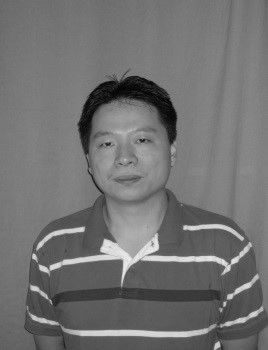
\includegraphics[width=1in,height=1.25in,clip,keepaspectratio]
{Photo/lpeng.png}}]{Lu Peng} 
received the bachelor’s and master’s
degrees in computer science and engineering from Shanghai Jiao Tong University, Shanghai,
China, and the Ph.D. degree in computer engineering from the University of Florida,
Gainesville, FL, USA.
He is the Gerard L. ''Jerry'' Rispone Professor with the Division of Electrical and Computer
Engineering, Louisiana State University, Baton Rouge, LA, USA. His current research interests
include memory hierarchy system, reliability, power efficiency, and other issues in processor
design.
Dr. Peng was a recipient of the ORAU Ralph E. Power Junior Faculty Enhancement Awards in 2007
and the Best Paper Award from IEEE International Green and Sustainable Computing Conference
(IGSC) in 2019 and IEEE International Conference on Computer Design (ICCD) processor
architecture track in 2001. He is a senior member of the IEEE and the ACM.
\end{IEEEbiography}


\EOD

\end{document}
